\chapter{Sun}
\label{ch:energy}

\section{Why this chapter comes first}

Chapter~\ref{ch:premises} named electricity the binding constraint. It is worth
being concrete about what that means, because it is not a figure of speech.

Cuban water is pumped, so no power means no water. Cuban food is refrigerated in
a climate where meat spoils in hours, so no power means the cold chain fails and
the food is lost between the field and the plate. Hospitals cannot run a surgical
list against a schedule of outages. A hotel without power or water does not merely
disappoint a guest; it produces the review that removes the next fifty guests. A
remote worker with no electricity has no job. A bakery with no electricity does
not bake. And a grid that has failed as a system four times fails more easily
each time, because every black start damages equipment and every restoration is
attempted with a fleet in worse condition than the last.

So the ordering in Part III is not a preference. Every sector chapter after this
one is conditional on it.

\section{Where the grid is}

Cuban generation is a small number of large oil-fired thermal units, most
commissioned between the 1960s and the 1980s, running past their design lives on
heavy, high-sulphur domestic crude they were not designed to burn, without
spares and frequently without fuel. Alongside them sit the distributed diesel and
fuel-oil sets installed in the Energy Revolution of 2006, now twenty years old,
and a set of floating Turkish power barges hired at hard-currency rates the
country struggles to pay.

In a normal pre-crisis year the system generated on the order of 20 terawatt-
hours and peaked around 3,000 to 3,300 megawatts.\unv{} By 2023 gross
generation was down to 15.3 terawatt-hours, and consumption per head had fallen
from about 1,856 kilowatt-hours in 2018 to 1,387 --- a quarter less electricity
per person in five years, which is not conservation but rationing. Through 2023--25 the
daily shortfall routinely ran a third of demand or more, with blackouts of twelve
to twenty hours outside Havana, and the national grid collapsed entirely in
October, November and December of 2024 and again in 2025.

The fuel is the recurring cost that matters. At the fleet's thermal efficiency
--- somewhere near 30 per cent --- 20 terawatt-hours of electricity requires
roughly six million tonnes of fuel oil equivalent a year. Cuba produces
perhaps half of that domestically, as heavy crude suitable for little else, and
must buy the rest --- which is why the electricity system, the balance of
payments and the political relationship with whoever is supplying the oil have
been the same problem since 1960.

\section{The resource, and the arithmetic}

Cuba sits between 20 and 23 degrees north with high, even insolation and very
little seasonal variation: global horizontal irradiance around 5.0 to 5.5
kilowatt-hours per square metre per day, which for a well-built fixed-tilt
photovoltaic system in a hot, humid climate yields something in the range of
1,500 to 1,700 kilowatt-hours per installed kilowatt-peak per year after
temperature derating and system losses \citep{gsa}.\unv{} The absence of a winter is worth
more than the peak irradiance: a Cuban array in January produces most of what it
produces in June, which removes the seasonal storage problem that dominates
temperate-latitude planning.

What it does not remove is the daily one. Cuban demand peaks between about six
and ten in the evening, when air conditioning, cooking and lighting coincide and
the sun has set. \emph{This is a storage problem at least as much as a
generation problem} (Fig.~\ref{fig:solar}a), and any programme that installs photovoltaics without
storage will find that it has displaced midday fuel, which is the cheapest fuel
to displace, and left the evening --- the hours that determine whether the grid
holds --- exactly as it was.

\begin{figure}[t]
\centering
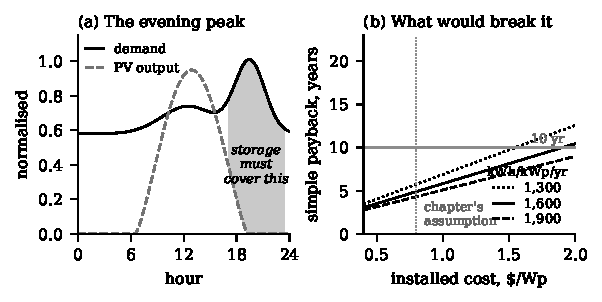
\includegraphics[width=\linewidth]{figs/solar}
\caption{(a)~Why the storage is not optional. Cuban demand peaks after sunset,
so photovoltaic capacity on its own displaces midday fuel --- the cheapest fuel
to displace --- and leaves the hours that decide whether the grid holds exactly
as they were. The load shape here is schematic; obtaining Cuba's actual hourly
demand curve is the first thing that should be done to this chapter, and
\texttt{verify.md} records it. (b)~The sensitivity the case actually turns on.
Below roughly \$1.50 per watt-peak the programme pays for itself inside a
decade across the whole plausible range of Cuban yields; above it, the argument
weakens and would need to be remade on grounds other than fuel saving.
Generated by \texttt{figs/solar.py}.}
\label{fig:solar}
\end{figure}

Here is the calculation, with its assumptions on the page so that a reader can
change them.

\begin{center}
\footnotesize
\begin{tabular}{@{}L{2.35in}r@{}}
\toprule
Target: half of a 20~TWh year from PV & 10~TWh/yr \\
Specific yield (assumed, conservative) & 1{,}600~kWh/kWp/yr \\
\midrule
Capacity required & $\approx$~6~GWp \\
Land at 1.5~ha/MWp & $\approx$~90~km$^2$ \\
\quad share of Cuban territory & $\approx$~0.08\% \\
Capital at \$0.80/Wp & $\approx$~\$5~bn \\
Evening storage, 4~h $\times$ 2~GW & 8~GWh \\
Storage at \$200/kWh & $\approx$~\$1.6~bn \\
\midrule
Total capital, over a decade & \$6--8~bn \\
Fuel displaced at 30\% efficiency & $\approx$~3~Mt/yr \\
Its value at \$400--500/t & \$1.2--1.5~bn/yr \\
\midrule
Simple payback & 5--6 years \\
\bottomrule
\end{tabular}
\end{center}

\noindent Every figure above is an order of magnitude; each is marked unverified
in the manuscript and listed in \texttt{verify.md}. Three things are
deliberately excluded and would
raise the cost: transmission and distribution reinforcement, which Cuba needs
anyway and which is a large number; the thermal fleet, which must be kept
running for firm capacity through the whole transition and therefore still needs
fuel, spares and maintenance; and the cost of capital, which for a defaulted
sovereign is the hardest input in the table and the reason
Chapter~\ref{ch:money}'s debt normalisation is a precondition rather than a
parallel exercise.

But the shape of the answer survives all of that, and the shape is the point.
The land requirement is a rounding error --- less than a tenth of one per cent
of the country, against something between one and two million hectares currently
under \emph{marab\'u} scrub. The capital cost is large but is of the same order
as a decade of the fuel bill it eliminates. And the recurring saving is in
foreign exchange, which is the scarcest thing Cuba has, converting the country's
largest recurring hard-currency cost into a domestic asset with no fuel input at
all.

That is the case, and it is a strong one. It was not a strong one in 2010, when
modules cost five times as much and batteries fifteen. The reason to do this now
is that the arithmetic changed.

\section{Hurricanes}

This is the design constraint that most solar advocacy for the Caribbean omits,
and omitting it is how a country spends five billion dollars and loses it in an
afternoon.

Cuba is hit by major hurricanes regularly and will be hit by stronger ones. The
lesson available from Puerto Rico after Mar\'ia in 2017 is specific and
usable: photovoltaic installations failed at very different rates depending on
how they were engineered, and the failures were overwhelmingly mounting failures
--- racking, fasteners, tracker stow --- rather than module failures. Systems
built to genuine high-wind specification largely survived; systems built to
mainland-United States standard specification largely did not.

\begin{design}{Building for the storm}
\label{d:storm}
\begin{rules}
\rl{1}{Specification} All installations are engineered to Category~5 wind
loading as a minimum, with mounting, fastening and foundation design certified
to that standard, and the certification published. This adds materially to
capital cost and is not optional; the alternative is to pay for the array twice.

\rl{2}{Distribution} Capacity is distributed across provinces and across many
sites rather than concentrated in a few large parks. A hurricane is a spatially
correlated risk, and the entire point of moving off a fleet of six large thermal
plants is not to rebuild that concentration in photovoltaics.

\rl{3}{Rooftops count double} Distributed rooftop generation on hospitals,
pumping stations, bakeries, telecoms sites and cold stores is resilient in a way
central capacity is not: it survives transmission damage, which is what actually
fails in a Cuban hurricane, and it keeps the critical load running while the grid
is restored.

\rl{4}{Spares held, not ordered} A national inventory of modules, inverters,
racking components and cable is held in country, in hardened storage, sized
against a modelled event. Post-storm procurement by a country with no credit
takes months.

\rl{5}{Self-insurance} Commercial insurance for Cuban assets is expensive and
in many markets unobtainable. The stabilisation fund of
Design~\ref{d:rentrule} carries an explicit reserve against grid and generation
losses, and the reserve is sized and published.
\end{rules}
\end{design}

\section{Who is allowed to own a generator}

The technology is the easy part. The reason Cuba has almost no distributed
generation despite a decade of favourable economics is legal: the national
electricity utility is a monopoly, private generation is permitted narrowly and
by permission, there is no bankable framework under which an independent producer
can sell power, and until very recently a household or private business had no
right to install a panel and use what it produced.

The solar parks now being installed with Chinese financing are the right
technology inside the wrong institution: capacity procured centrally, owned by
the state, connected to a grid the state runs, financed by a bilateral
relationship of exactly the kind Chapters~\ref{ch:sovieteconomy} and
\ref{ch:venezuela} warned about. They will help. They will not, by themselves,
solve this, and they do nothing at all about the evening peak.

\begin{design}{Generation rights}
\label{d:genrights}
\begin{rules}
\rl{1}{Rooftop by right} Any owner or lawful occupier may install generation and
storage on their own premises and consume what it produces, without permission,
subject only to published safety and interconnection standards. Not by licence,
not by category, not by application --- by right, per Design~\ref{d:commit}.2.

\rl{2}{Net billing} Surplus exported to the grid is purchased at a published
tariff set by the regulator, paid in the currency of Design~\ref{d:regime}, with
settlement periods fixed in regulation. Net \emph{billing} rather than net
metering, because the value of exported midday power is genuinely lower than the
value of consumed evening power and pretending otherwise builds a subsidy that
later has to be withdrawn.

\rl{3}{Independent producers} A standard-form power purchase agreement,
published, non-negotiable in its core terms, with international arbitration and
a payment guarantee. A one-off negotiated PPA in a country with Cuba's payment
record is not bankable; a standard instrument with a guarantee behind it can be.

\rl{4}{Regulator} An independent energy regulator with the tenure, budget and
publication obligations of Design~\ref{d:courts}, separate from the utility it
regulates and from the ministry that owns the utility. At present the operator,
the owner, the planner and the regulator are the same entity, which is the same
conflict of interest Chapter~\ref{ch:life} identifies in pharmaceuticals.

\rl{5}{Unbundling, eventually} Transmission and system operation separated from
generation, with open, non-discriminatory access to the network. This is a later
phase --- it is hard, and doing it badly is worse than not doing it --- but it
is stated here because the interconnection standards written in phase one
determine whether it is possible in phase three.

\rl{6}{Import freedom} Panels, inverters, batteries, cable and mounting hardware
enter free of duty and without licence, for anybody. Cuba currently has a
population willing to buy its own solar equipment with remittance money and a
customs regime that makes doing so an ordeal. This clause costs the state
nothing and is the single fastest megawatt available.
\end{rules}
\end{design}

\section{Biomass, and what is left of sugar}

Bagasse --- the fibre left after cane is crushed --- is the one dispatchable
renewable Cuba already knows how to burn, and the 2020 plant at Ciro Redondo
demonstrated that a modern bagasse unit can export power to the grid rather than
merely running its own mill.

The problem is that the resource has gone. Chapter~\ref{ch:crisis} recorded a
harvest in the low hundreds of thousands of tonnes; there is no bagasse because
there is no cane. So biomass in Cuba is hostage to a decision that belongs to
Chapter~\ref{ch:land}, and this chapter should not plan around a feedstock whose
existence depends on reviving an industry that mostly is not coming back.

What is available regardless is \emph{marab\'u}. The thorny scrub that has taken
over between one and two million hectares of Cuban farmland is a dense hardwood,
it already supports a small charcoal export, and clearing it serves two purposes
at once --- it recovers agricultural land and it produces fuel. It is not a
large power resource and should not be sold as one. It is a genuine transitional
one, and it is the rare case where the disposal cost of a problem is negative.

\section{The order of operations}

The last section, and the most important, because a five-billion-dollar
programme takes a decade and Cuba's problem is now.

\emph{Before anything is built.} The cheapest megawatt is the one not consumed,
and the second cheapest is the one not lost on the way. In 2023 Cuba generated
15.3 terawatt-hours and lost 3.7 of them --- close to a quarter --- in
transmission and distribution before they reached a customer.\unv{} That is an
extraordinary figure by any standard, and it means that repairing the network
delivers usable energy at a fraction of the cost per kilowatt-hour of building
new capacity to generate power that will then be lost in the same wires.

Alongside it, demand. Cuba has done this before and done it well: the 2006
programme replaced nine million incandescent bulbs and millions of inefficient
appliances and cut consumption measurably. Two decades on the appliance stock is
old again and the same intervention is available at lower cost with better
technology. Efficient lighting, refrigeration and air conditioning, industrial
motor replacement, and loss reduction are all faster, cheaper and less
capital-hungry than generation, and they can begin in month one. A programme
that goes straight to building solar parks while a quarter of the output leaks
out of the network is buying generation it will not be able to deliver.

\emph{Critical loads first.} Before utility-scale anything, put photovoltaics
and batteries on the loads whose failure is catastrophic rather than merely
expensive: hospitals, water pumping stations, cold stores, bakeries, telecoms.
These are small, fast, high-value, hurricane-resilient, and they buy the
programme public support that a distant solar park does not.

\emph{Keep the thermal fleet alive.} This is unglamorous and unavoidable. The
existing plants must provide firm capacity for the whole of the transition, which
means fuel, spares and maintenance have to be funded now, at the same time as
the new capacity is being financed. A plan that starves the old fleet to pay for
the new one produces a worse blackout in year three.

\emph{Then capacity, with storage, distributed.} Per the arithmetic above and
Designs~\ref{d:storm} and \ref{d:genrights}, over roughly a decade, with the
storage procured alongside the generation and not after it.

\begin{design}{The energy sequence}
\label{d:energyseq}
\begin{rules}
\rl{1}{Months 0--6} Import liberalisation for equipment (Design~\ref{d:genrights}.6);
rooftop rights by decree; efficiency programme launched; critical-load
installations begun; fuel and spares for the existing fleet funded as a first
call on the budget.

\rl{2}{Months 6--24} Regulator established; standard PPA published; net billing
tariff set; interconnection standards issued; first independent producer
tenders, competitively bid with published results per
Chapter~\ref{ch:integrity}.

\rl{3}{Years 2--10} Roughly 6~GWp and 8~GWh built out, distributed across
provinces, with the eastern provinces weighted first --- they have the worst
supply, the most land and the least political voice, and per
Design~\ref{d:municipal}.2 the design does not let the benefits accrue where the
tourists are.

\rl{4}{Throughout} No preferential allocation of capacity, fuel, currency or
grid access to any state or military-linked entity. Energy is where Cuban
discretion has been most valuable and therefore most corrupting, and
Chapter~\ref{ch:integrity} treats generation procurement as a priority
publication target.
\end{rules}
\end{design}
